% Writed by: Stavros Papantonakis
%
%!TEX TS-program = xelatex
%!TEX encoding = UTF-8 Unicode
%
\setcounter{section}{1}
\section{Γενικό Πλαίσιο}


\noindent
Ο αλγόριθμος RSA περιλαμβάνει υπολογισµούς σε µεγάλους αριθµούς. Αυτοί οι υπολογισµοί
δεν µπορούν να διεξαχθούν απευθείας στη µηχανή χρησιµοποιώντας απλούς αριθµητικούς
τελεστές σε προγράµµατα, επειδή αυτοί οι τελεστές µπορούν να λειτουργήσουν µόνο σε
κλασικούς τύπους δεδοµένων, όπως ακέραιους 32 bit και 64 bit. Οι αριθµοί που εµπλέκονται
στους αλγόριθµους RSA είναι τυπικά µεγαλύτεροι από 512 bit. Για παράδειγµα, για να
πολλαπλασιάσουµε δύο αριθµούς ακέραιους 32-bit a και b, πρέπει απλώς να χρησιµοποιήσουµε
a*b στο πρόγραµµά µας. Ωστόσο, εάν οι αριθµοί είναι µεγάλοι, δε µπορούµε να το κάνουµε
αυτό. Αντίθετα, πρέπει να χρησιµοποιήσουµε έναν αλγόριθµο (δηλαδή µια συνάρτηση) για να
υπολογίσουµε τα γινόµενά τους και θα µας επιτρέψει έτσι να ξεπεράσουµε τα όρια της µηχανής
και συγκεκριµένα των κυκλωµάτων της αριθµητικής και λογικής µονάδας της.

\noindent
Υπάρχουν διάφορες βιβλιοθήκες που µπορούν να εκτελούν αριθµητικές πράξεις σε ακέραιους
αριθµούς αυθαίρετου µεγέθους. Σε αυτό το εργαστήριο, θα χρησιµοποιήσουµε τη βιβλιοθήκη
µεγάλων αριθµών που παρέχεται από το openssl. Για να χρησιµοποιήσετε αυτήν τη βιβλιοθήκη,
θα ορίσουµε κάθε µεγάλο αριθµό ως τύπο BIGNUM και, στη συνέχεια, θα χρησιµοποιήσουµε
τα API που παρέχει η βιβλιοθήκη για διάφορες λειτουργίες, όπως πρόσθεση, πολλαπλασιασµό,
ύψωση σε δύναµη, αριθµητική υπολοίπου κ.λπ.

\noindent
Στην άσκηση αυτή θα χρησιµοποιηθεί όλο το υλικό του θεωρητικού µέρους του µαθήµατος για
τον RSA που είναι ανεβασµένο στο eclass.

\subsection{BIGNUM APIs}
\noindent
Όλα τα APIs για µεγάλους αριθµούς µπορούν να βρεθούν στο\\ \url{https://linux.die.net/man/3/bn}. Στη συνέχεια περιγράφονται µερικά από τα APIs που χρειάζονται για την
εργαστηριακή αυτή άσκηση.

\noindent
Ορισµένες συναρτήσεις της βιβλιοθήκης απαιτούν προσωρινές µεταβλητές. Δεδοµένου ότι η
δυναµική κατανοµή µνήµης για τη δηµιουργία των BIGNUMs είναι αρκετά δαπανηρήόταν χρησιµοποιείται σε συνδυασµό µε επαναλαµβανόµενες κλήσεις υπορουτίνας,
δηµιουργείται µια δοµή BNX CTX για να κρατάει προσωρινές µεταβλητές BIGNUM που
χρησιµοποιούνται από συναρτήσεις βιβλιοθήκης. Πρέπει να δηµιουργήσουµε µια τέτοια
δοµή και να τη µεταβιβάσουµε (περάσουµε) στις συναρτήσεις που την απαιτούν.
\begin{center}
	\begin{lstlisting}	
BN_CTX *ctx = BN_CTX_new ()	
	\end{lstlisting}	
\end{center}

\noindent
Αρχικοποίηση της µεταβλητής BIGNUM
\begin{center}
	\begin{lstlisting}	
BIGNUM *a = BN_new()	
	\end{lstlisting}	
\end{center}

\noindent
Υπάρχουν πολλοί τρόποι να εκχωρηθεί µια τιµή σε µία BIGNUM µεταβλητή.
\begin{center}
	\begin{lstlisting}	
// Assign a value from a decimal number string
BN_dec2bn(&a, “12345678901112231223");
// Assign a value from a hex number string
BN_hex2bn(&a, “2A3B4C55FF77889AED3F");
// Generate a random number of 128 bits
BN_rand(a, 128, 0, 0);
// Generate a random prime number of 128 bits
BN_generate_prime_ex(a, 128, 1, NULL, NULL, NULL);	
	\end{lstlisting}	
\end{center}

\noindent
Εκτύπωση ενός µεγάλου αριθµού.
\begin{center}
	\begin{lstlisting}	
void printBN(char *msg, BIGNUM * a)
{
	// Convert the BIGNUM to number string
	char * number_str = BN_bn2dec(a);
	// Print out the number string
	printf("%s %s\n", msg, number_str);
	// Free the dynamically allocated memory
	OPENSSL_free(number_str);
}	
	\end{lstlisting}	
\end{center}

\noindent
Υπολογισµός \(res = a − b και res = a + b:\)
\begin{center}
	\begin{lstlisting}	
BN_sub(res, a, b);
BN_add(res, a, b);	
	\end{lstlisting}	
\end{center}


\noindent
Υπολογισµός \(res = a * b.\) Απαιτείται µία BN CTX δοµή σε αυτό το API.
\begin{center}
	\begin{lstlisting}	
		BN_mul(res, a, b, ctx)
	\end{lstlisting}	
\end{center}

\noindent
Υπολογισµός \(res = a * b * mod(n):\)
\begin{center}
	\begin{lstlisting}	
BN_mod_mul(res, a, b, n, ctx)	
	\end{lstlisting}	
\end{center}

\noindent
Υπολογισµός \(res = a^c * mod(n):\)
\begin{center}
	\begin{lstlisting}	
BN_mod_exp(res, a, c, n, ctx)	
	\end{lstlisting}	
\end{center}

\noindent
Υπολογισµός αντίστροφου, δηλαδή, για ένα a να βρεθεί b, τέτοιο ώστε \(a * b * mod(n) = 1
(a * b ≡ 1 * mod(n))\). Η τιµή b καλείται ο αντίστροφος του a, στην αριθµητική υπολοίπου
n και υπάρχει µόνο αν gcd(a,b)=1.
\begin{center}
	\begin{lstlisting}	
BN_mod_inverse(b, a, n, ctx);
	\end{lstlisting}	
\end{center}

\subsection{Παράδειγμα}

\noindent
Στη συνέχεια παρουσιάζεται ένα ολοκληρωµένο παράδειγµα. Σε αυτό, αρχικοποιούµε τρεις
BIGNUM µεταβλητές, a, b, και n, και στη συνέχεια υπολογίζουµε το \(a*b\) και το \((a * b * mod(n)\).
Υπάρχουν πολλοί τρόποι να εκχωρηθεί µια τιµή σε µία BIGNUM µεταβλητή.
\begin{center}
	\begin{lstlisting}	
/* bn_sample.c */
#include <stdio.h>
#include <openssl/bn.h>
#define NBITS 256
void printBN(char *msg, BIGNUM * a)
{
	/* Use BN_bn2hex(a) for hex string
	* Use BN_bn2dec(a) for decimal string */
	char * number_str = BN_bn2hex(a);
	printf("%s %s\n", msg, number_str);
	OPENSSL_free(number_str);
}
	
int main ()
{
	BN_CTX *ctx = BN_CTX_new();
	
	BIGNUM *a = BN_new();
	BIGNUM *b = BN_new();
	BIGNUM *n = BN_new();
	BIGNUM *res = BN_new();
	
	// Initialize a, b, n
	BN_generate_prime_ex(a, NBITS, 1, NULL, NULL, NULL);
	BN_dec2bn(&b, "273489463796838501848592769467194369268");
	BN_rand(n, NBITS, 0, 0);
	
	// res = a*b
	BN_mul(res, a, b, ctx);
	printBN("a * b = ", res);
	
	// res = a^b mod n
	BN_mod_exp(res, a, b, n, ctx);
	printBN("aˆc mod n = ", res);
	return 0;
}	
	\end{lstlisting}	
\end{center}

Μεταγλώττιση: Για τη µεταγλώττιση του προγράµµατος bn\_sample.c χρησιµοποιείστε την
παρακάτω εντολή
\begin{center}
	\begin{lstlisting}	
$ gcc bn_sample.c -lcrypto
	\end{lstlisting}	
\end{center}

\section{Δραστηριότητες Εργαστηρίου}
\noindent
Για την αποφυγή λαθών θα πρέπει να αντιγράφετε τους αριθµούς που θα συναντήσετε
παρακάτω και όχι να τους πληκτρολογείτε. Στην άσκηση που θα παραδώσετε θα πρέπει να
συµπεριλάβετε τα βήµατα που ακολουθήσατε, τον κώδικα, και τα αποτελέσµατα που πήρατε
όταν τον τρέξατε.

\subsection{Δραστηριότητα 1: Δηµιουργώντας το ιδιωτικό κλειδί}
\noindent
Έστω p και q δύο πρώτοι αριθµοί και e ένας αριθµός. Έστω n = p * q. Θα χρησιµοποιήσουµε το
(e, n) ως το δηµόσιο κλειδί. Υπολογίστε το ιδιωτικό κλειδί d. Οι δεκαεξαδικές τιµές των p, q, και
e αναφέρονται παρακάτω. Πρέπει να σηµειωθεί ότι αν και τα p και q που χρησιµοποιούνται σε
αυτό τη δραστηριότητα είναι αρκετά µεγάλοι αριθµοί, δεν είναι αρκετά µεγάλοι για να είναι
ασφαλείς. Προφανώς τα κάνουµε µικρά για λόγους απλότητας. Στην πράξη, αυτοί οι αριθµοί
θα πρέπει να έχουν µήκος τουλάχιστον 512 bits (αυτός που χρησιµοποιείται εδώ είναι µόνο 128
bits).

\begin{lstlisting}	
p = F7E75FDC469067FFDC4E847C51F452DF
q = E85CED54AF57E53E092113E62F436F4F
e = 0D88C3
\end{lstlisting}


\subsection*{Απάντηση:}
\noindent
Στην ασύμμετρη κρυπτογράφηση χρησιμοποιούνται δυο κλειδιά κρυπτογράφησης, ένα Ιδιωτικό (Privet Key)
που είναι γνωστό μόνο στον ιδιοκτήτη του και ένα Δημόσιο (Public Key) που διατίθεται προς όλους.
η σχέση των κλειδιών είναι τέτοια έτσι ώστε όταν κρυπτογραφηθεί κάτι με το ένα να αποκρυπτογραφηθεί 
αποκλειστικά μόνο με το άλω. Το κάθε κλειδί από αυτά αποτελείτε από ένα ζεύγος αριθμόν. Για παράδειγμα 
το Δημόσιο κλειδί αποτελείτε από το ζευγάρι των ακεραίων (e,n) και το Ιδιωτικό από το (d,n). Το n προκύπτει
από το γινωμένο δυο πολύ μεγάλων πρώτων αριθμών p και q. Το e είναι επίσης πρώτος αριθμός και επιλέγετε έτσι ώστε να μην έχει κοινούς παράγοντες με το (p-1)*(q-1). Τέλος για το d η επιλογή γίνεται έτσι ώστε
\begin{center}
	\textbf{	\Large \(e * d \equiv 1 * mod((p - 1)*(q-1)) \Rightarrow e * d *mod((p - 1)*(q-1))=1 \)}	
\end{center}
\noindent
Επομένως για να υπολογίσουμε το ιδιωτικό μας κλειδί θα χρησιμοποιήσουμε μερικά από τα \textbf{BIGNUM APIs}
για να δηλώσουμε μεταβλητές τύπου \textbf{BIGNUM} καθώς και να τους εκχωρήσουμε τιμές.
Αρχικά δηλώνουμε της p,q,e,n,d της οποίες θα χρειαστούμε για των υπολογισμό του κλειδιού 
δηλώνουμε μια εξτρα μεταβλητή one για να αποθηκεύσουμε τον αριθμό 1. Αυτό το κάνουμε γιατί 
η συνάρτηση BN\_sub() δέχεται ως ορίσματα μόνο \textbf{BIGNUM} μεταβλητές. Στην Συνεχεία 
δηλώνουμε τα q\_minus\_1, p\_minus\_1 και τέλος την n\_res. Είμαστε πλέων έτοιμοι για να 
αστικοποιήσουμε της τιμές που μας δίνονται με την συνάρτηση BN\_hex2bn(). Υπολογίζουμε το n και 
τα q-1, p-1 καθώς και το γινόμενο τους, οπού το αποτέλεσμα του το αποθηκεύουμε στην n\_res. Τέλος 
με την συνάρτηση BN\_mod\_inverse() υπολογίζουμε το τελικό d.


\begin{center}
			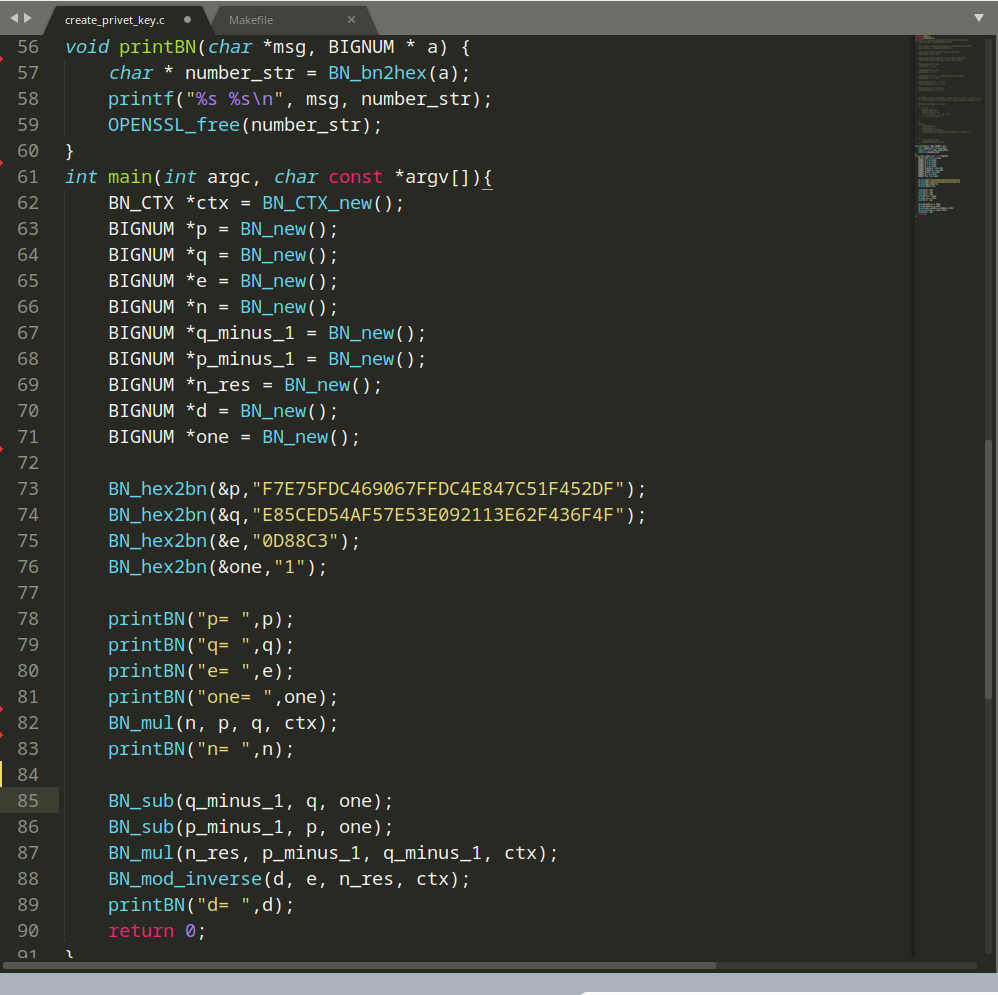
\includegraphics[width=1\textwidth]{image/image31code.PNG}		
\end{center}
\begin{center}
			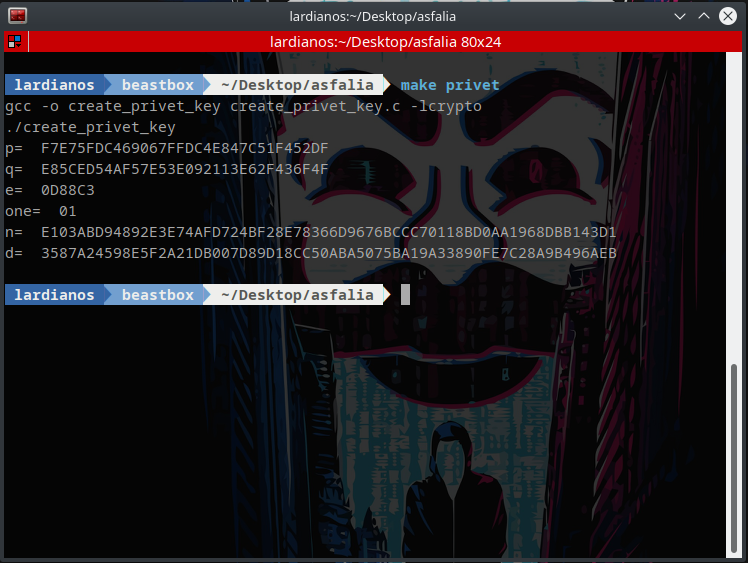
\includegraphics[width=1\textwidth]{image/image31term.PNG}		
\end{center}


\subsection{Δραστηριότητα 2: Κρυπτογράφηση µηνύµατος}
\noindent
Έστω (e, n) το δηµόσιο κλειδί. Κρυπτογραφήστε το µήνυµα “A top secret!" (χωρίς τα
εισαγωγικά). Πρέπει να µετατρέψουµε αυτή την συµβολοσειρά ASCII σε µια δεκαεξαδική
συµβολοσειρά και, στη συνέχεια, να µετατρέψουµε την δεκαεξαδική συµβολοσειρά σε BIGNUM
χρησιµοποιώντας το hex-to-bn API BN\_hex2bn(). Η ακόλουθη εντολή python µπορεί να
χρησιµοποιηθεί για τη µετατροπή µιας απλής συµβολοσειράς ASCII σε µια δεκαεξαδική
συµβολοσειρά.

\begin{lstlisting}	
$ python -c 'print("A top secret!".encode("hex"))'

4120746f702073656372657421
\end{lstlisting}

Τα δηµόσια κλειδιά παρατίθενται παρακάτω (σε δεκαεξαδική µορφή). Παρέχουµε επίσης το
ιδιωτικό κλειδί d για να επαληθεύσετε το αποτέλεσµα της κρυπτογράφησης.
\enlargethispage{\baselineskip}
\begin{lstlisting}	
n = DCBFFE3E51F62E09CE7032E2677A78946A849DC4CDDE3A4D0CB81629242FB1A5
e = 010001 (this hex value equals to decimal 65537)
M = A top secret!
d = 74D806F9F3A62BAE331FFE3F0A68AFE35B3D2E4794148AACBC26AA381CD7D30D
\end{lstlisting}


\subsection*{Απάντηση:}
\noindent
Για την κρυπτογράφηση ενός μηνύματος χρειαζόμαστε το δημόσιο κλειδί του παραλήπτη, το 
οποίο μας δίνετε (e,n). Το μήνυμα που θα κρυπτογραφήσουμε θα είναι το "A top secret!".
Για να γνωρίζουμε ώμος ότι το μήνυμα κρυπτογραφήθηκε σωστά και ότι κρατήθηκε ακέραιο
κατά την διαδικασία της κρυπτογράφησης θα πρέπει να μπορέσουμε να το αποκρυπτογραφήσουμε.
Εφόσον κρυπτογραφηθεί με το δημόσιο κλειδί μπορεί να αποκρυπτογραφηθεί μόνο με το ιδιωτικό (d,n).

Για την κρυπτογράφηση ισχύει:
\begin{center}
	\textbf{	\Large \(C=M^emod(n)\)}	
\end{center}
Καθώς και για την αποκρυπτογράφηση:
\begin{center}
	\textbf{	\Large \(M=C^dmod(n)\)}	
\end{center}
\noindent

Αρχικά μετατρέπουμε το μήνυμα σε δεκαεξαδική μορφή. Έπειτα το εκχωρούμε σε μια μεταβλητή μαζί με τα
υπόλοιπα δεδομένα. Στην συνεχεία καλούμε την BN\_mod\_exp() με ορίσματα το μήνυμα σε δεκαεξαδική μορφή, το
δημόσιο κλειδί (e,n) και έναν \textbf{BN\_CTX} pointer. Αυτό μας επιστρέφει στην μεταβλητή crypto\_message το 
κρυπτογράφημα. Σε αυτό το σημείο δεν γνωρίζουμε αν το αποτέλεσμα που πήραμε είναι σωστό. για αυτόν τον λόγο
θα κάνουμε την ανάστροφη διαδικασία για να δούμε αν αποκρυπτογραφηθεί. θα χρησιμοποιήσουμε δηλαδή το ιδιωτικό
κλειδί (d,n) για να αποκρυπτογραφήσουμε το μήνυμα με τον ίδιο τρόπο, καλώντας την BN\_mod\_exp() άλλα αυτήν την φορά με ορίσματα οπός, το κρυπτογραφημένο μήνυμα το ιδιωτικό κλειδί (d,n) και τον \textbf{BN\_CTX} pointer. όπως παρατηρούμε το αποτέλεσμα είναι το αρχικό μήνυμα.
\begin{center}
			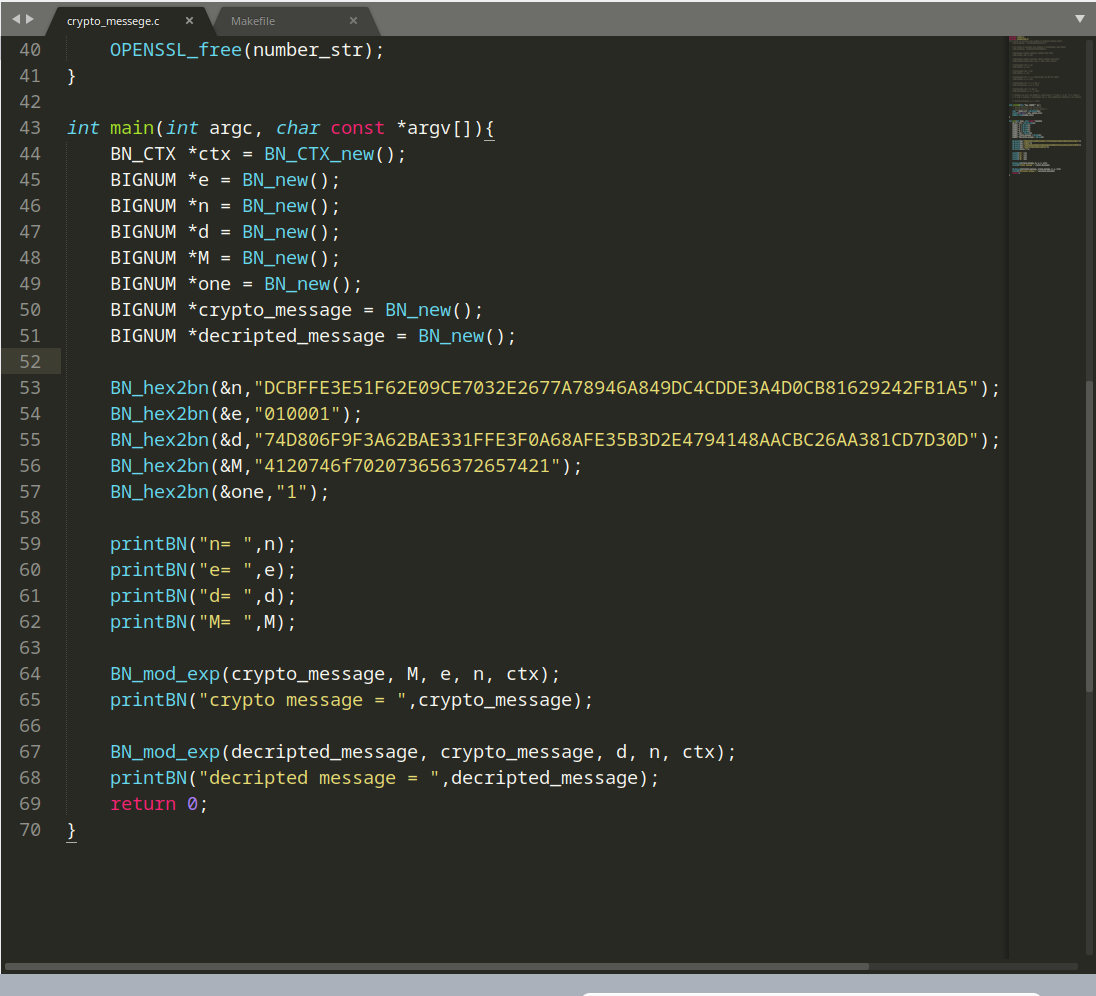
\includegraphics[width=0.9\textwidth]{image/image32code.PNG}		
\end{center}
\begin{center}
			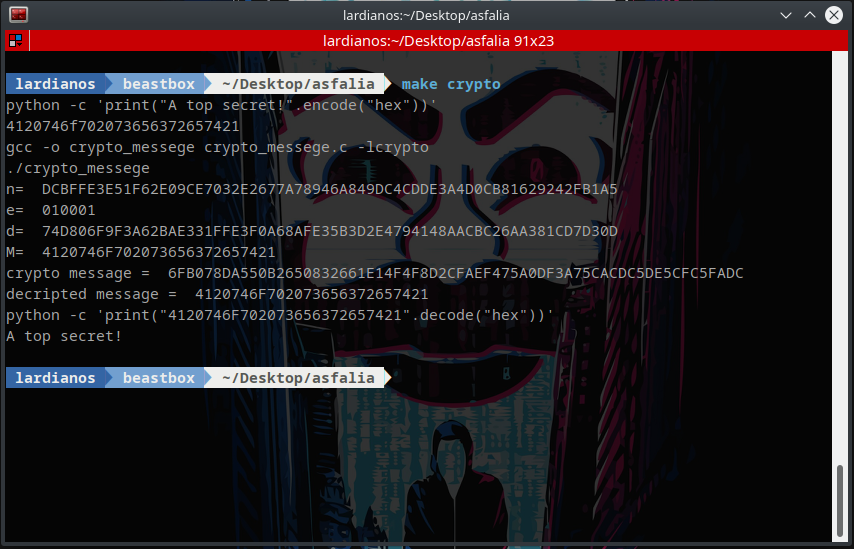
\includegraphics[width=0.9\textwidth]{image/image32term.PNG}		
\end{center}
\subsection{Δραστηριότητα 3: Αποκρυπτογράφηση µηνύµατος}
\noindent
Το δηµόσιο και το ιδιωτικό κλειδί που χρησιµοποιήθηκαν σε αυτή τη δραστηριότητα είναι τα
ίδια µε αυτά στη δραστηριότητα 2. Αποκρυπτογραφήστε το ακόλουθο κρυπτογράφηµα C, και
µετατρέψτε το πίσω σε µία ASCII συµβολοσειρά σε αναγνώσιµη µορφή.

\normalsize C = \small 8C0F971DF2F3672B28811407E2DABBE1DA0FEBBBDFC7DCB67396567EA1E2493F\\

\noindent
Μπορείτε να χρησιµοποιήσετε την παρακάτω εντολή python για να µετατρέψτε µία
δεκαεξαδική συµβολοσειρά πίσω σε µία ASCII συµβολοσειρά σε αναγνώσιµη µορφή.
\begin{lstlisting}	
$ python -c 'print("4120746f702073656372657421".decode("hex"))'

A top secret!
\end{lstlisting}

\subsection*{Απάντηση:}
\noindent
Εφόσον τα κλειδιά είναι ίδια με τα προηγούμενα για την αποκρυπτογράφηση αυτού του μηνύματος
θα εφαρμόσουμε την ίδια διαδικασία αποκρυπτογράφησης. μετατρέποντας την δεκαεξαδική συμβολοσειρά
σε ascii με την εντολή της python διαβάζουμε το μήνυμα που είχε κρυπτογραφηθεί.
\begin{center}
			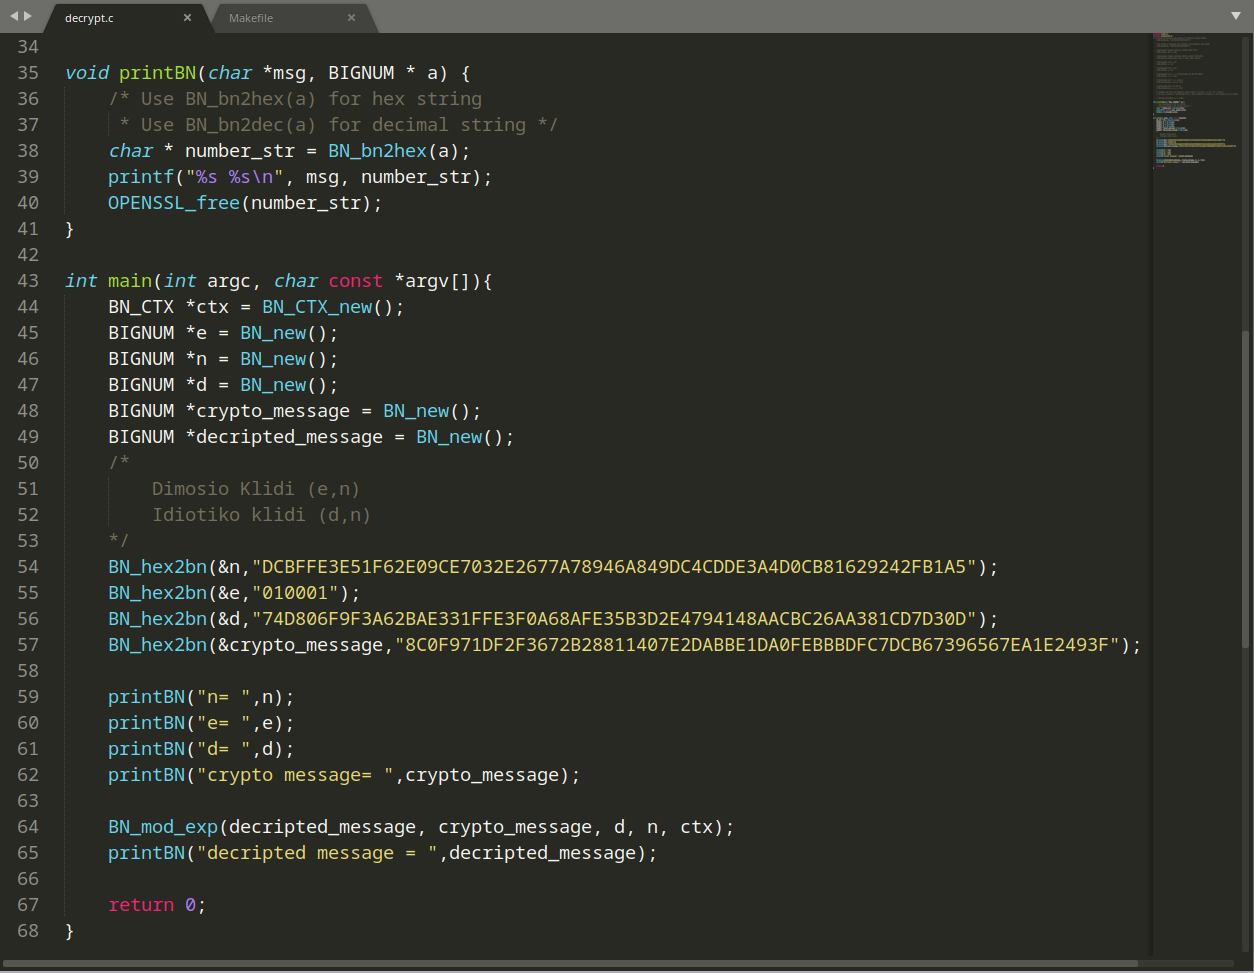
\includegraphics[width=1\textwidth]{image/image33code.PNG}		
\end{center}
\begin{center}
			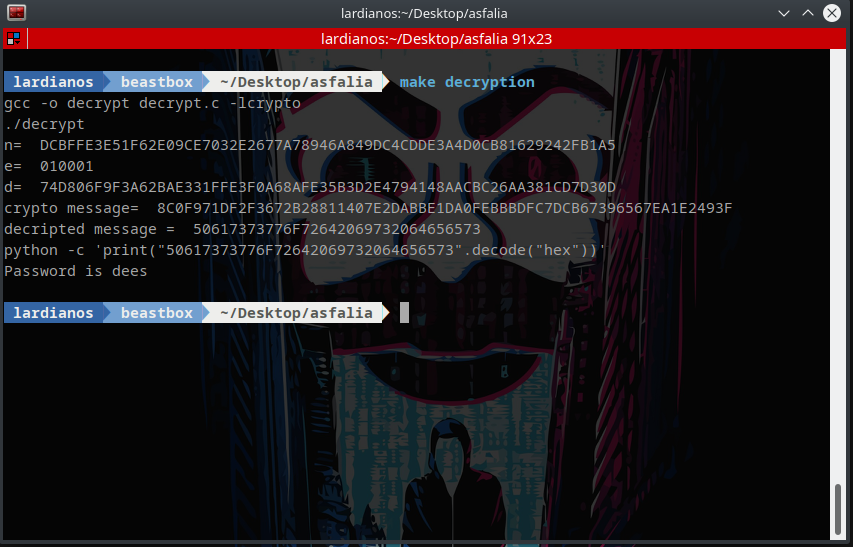
\includegraphics[width=1\textwidth]{image/image33term.PNG}		
\end{center}

\subsection{Δραστηριότητα 4: Υπογραφή µηνύµατος}
\noindent
Το δημόσιο και το ιδιωτικό κλειδί που χρησιμοποιήθηκαν σε αυτή τη δραστηριότητα είναι τα
ίδια µε αυτά στη δραστηριότητα 2. Δημιουργήστε µία υπογραφή για το ακόλουθο µήνυµα
(υπογράψτε απευθείας το µήνυµα αυτό αντί να υπογράψτε την τιµή κατακερµατισµού, hash
value):

\begin{lstlisting}
M = I owe you $2000.
\end{lstlisting}

\noindent
Μετά κάντε µία µικρή αλλαγή στο µήνυµα M, όπως να αλλάξετε το \$2000 σε \$3000, και
υπογράψτε το τροποποιηµένο µήνυµα. Συγκρίνετε τις υπογραφές και περιγράψτε τι
παρατηρείτε.

\subsection*{Απάντηση:}
\noindent
Εφόσον έχουμε κρυπτογραφήσει ένα μήνυμα με το δημόσιο κλειδί κάποιου και του το αποστείλουμε 
αυτός θα είναι ο μόνος που θα μπορεί να το αποκρυπτογράφηση, άλλα σε καμιά περίπτωση δεν θα μπορεί να 
είναι σίγουρος για το ποιος του το έχει αποστείλει. Με λίγα λογία έχουμε εξασφάλιση την 
\textbf{Ακεραιότητα(integrity)} του μηνύματος και την \textbf{Εμπιστευτικότητα(confidentiality)} άλλα
όχι την \textbf{Αυθεντικότητα(authentication)} και την \textbf{Μη άρνηση ταυτότητας (non-repudiation)}.
Για να τα εξασφαλίσουμε αυτά χρησιμοποιήσουμε την ψηφιακή υπογραφή. Η ψηφιακή υπογραφή είναι είτε ένα μέρος
του μηνύματος είτε ολόκληρο το μήνυμα είτε άπλα κάτι χαρακτηριστικό κρυπτογραφημένο με τω ιδιωτικό κλειδί
του αποστολέα και τοποθετημένο συνήθως στο τέλος του κρυπτογραφήματος. εφόσον είναι κρυπτογραφημένο
με το ιδιωτικό κλειδιά το αποστολέα μπορεί να αποκρυπτογραφηθεί μόνο από το δημόσιο του κλειδί. Με άπλα λογία 
μπορεί να αποκρυπτογραφηθεί από οποιονδήποτε έχει λάβει το μήνυμα και εφόσον αποκρυπτογραφηθεί από το δημόσιο
κλειδί του αποστολέα σημαίνει ότι ο μοναδικός που θα μπορούσε να το έχει κρυπτογραφήσει θα ήταν ο αποστολέας.
Έτσι μπορεί να εξασφαλιστεί και η αυθεντικότητα του μηνύματος άλλα και η μη άρνηση ταυτότητας.

\noindent
Αρχικά μετατρέπουμε το μήνυμα σε δεκαεξαδική μορφή με το \$2000 και το\$3000. Αν συγκρίνουμε τα αποτελέσματα
παρατηρούμε μια διάφορα ενός χαρακτήρα. κρυπτογραφώντας ώμος τα μηνύματα τα κρυπτογραφήματα είναι εντελώς
διαφορετικά.
\begin{center}
			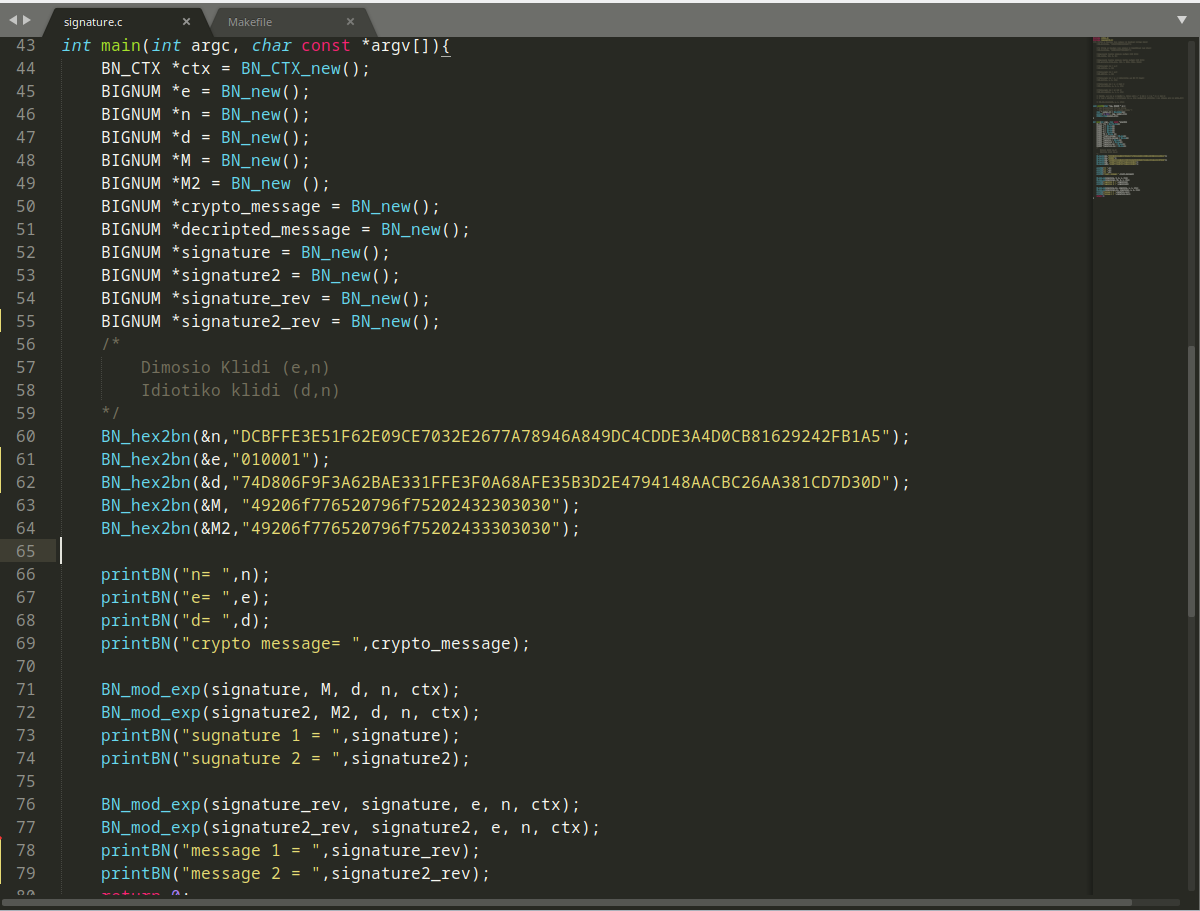
\includegraphics[width=1\textwidth]{image/image34code.PNG}		
\end{center}
\begin{center}
			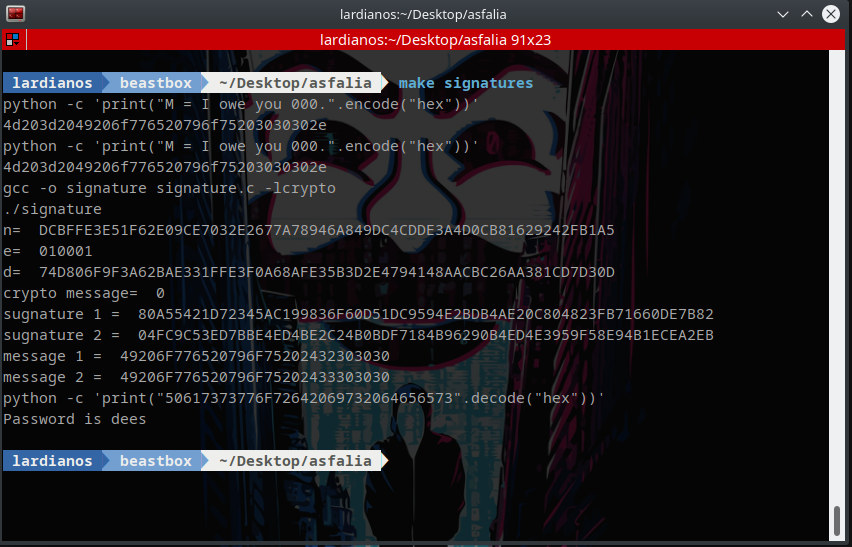
\includegraphics[width=1\textwidth]{image/image34term.PNG}		
\end{center}

\subsection{Δραστηριότητα 5: Επαλήθευση Υπογραφής}
\noindent
Ο Bob λαµβάνει ένα µήνυµα Μ = “Launch a missile.” από την Alice, µε την υπογραφή της S.
Γνωρίζουµε ότι το δηµόσιο κλειδί της Alice είναι το (e, n). Επιβεβαιώστε ότι η υπογραφή είναι
της Alice ή όχι. Το δηµόσιο κλειδί και η υπογραφή (σε δεκαεξαδική µορφή) δίνονται παρακάτω:

\begin{lstlisting}

M = Launch a missle.
S = 643D6F34902D9C7EC90CB0B2BCA36C47FA37165C0005CAB026C0542CBDB6802F
e = 010001 (this hex value equals to decimal 65537)
n = AE1CD4DC432798D933779FBD46C6E1247F0CF1233595113AA51B450F18116115
\end{lstlisting}

\noindent
Θεωρείστε ότι η υπογραφή έχει αλλοιωθεί (καταστραφεί), έτσι ώστε το τελευταίο byte της
υπογραφής να αλλάζει από 2F σε 3F, δηλαδή, υπάρχει µόνο ένα bit που έχει αλλάξει.
Επαναλάβατε τη δραστηριότητα αυτή και περιγράψτε τι θα συµβεί κατά τη διαδικασία
επαλήθευσης της υπογραφής.

\subsection*{Απάντηση:}
\noindent
Λαμβάνοντας ο bob το μήνυμα με την ψηφιακή υπογραφή το μόνο που έχει να κάνη για να επιβεβαίωση ότι
του το έστειλε η alice είναι να χρησιμοποίηση το δημόσιο κλειδί της για να την αποκρυπτογραφήσει.
Αποκρυπτογραφώντας το παρατηρούμε μια δεκαεξαδική συμβολοσειρά χρησιμοποιώντας και πάλι την εντολή
της python είτε για να μετατρέψουμε το μήνυμα σε δεκαεξαδικό είτε για να μετατρέψουμε το αποκρυπτογραφημένο
δεκαεξαδικό σε ascii. παρατηρούμε ότι είναι ακριβώς τα ίδια, επόμενος σίγουρα αυτό το μήνυμα το έστειλε
η alice

\noindent
Αλλάζοντας μόνο ένα bit από την ψηφιακή υπογραφή παρατηρούμε ότι η συμβολοσειρά που προκύπτει
από τη αποκρυπτογραφήσει είναι εντελώς άσχετη με το αρχικό μήνυμα και δεν βγάζει κανένα νόημα 
αν την μετατρέψουμε σε ascii. αυτό σημαίνει ότι αν η ψηφιακή υπογραφή αλλοιωθεί τότε δεν θα βγάζει
κανένα αποτέλεσμα, κάτι που μας εξασφαλίζει την ακεραιότητα ενός μηνύματος 

\begin{center}
			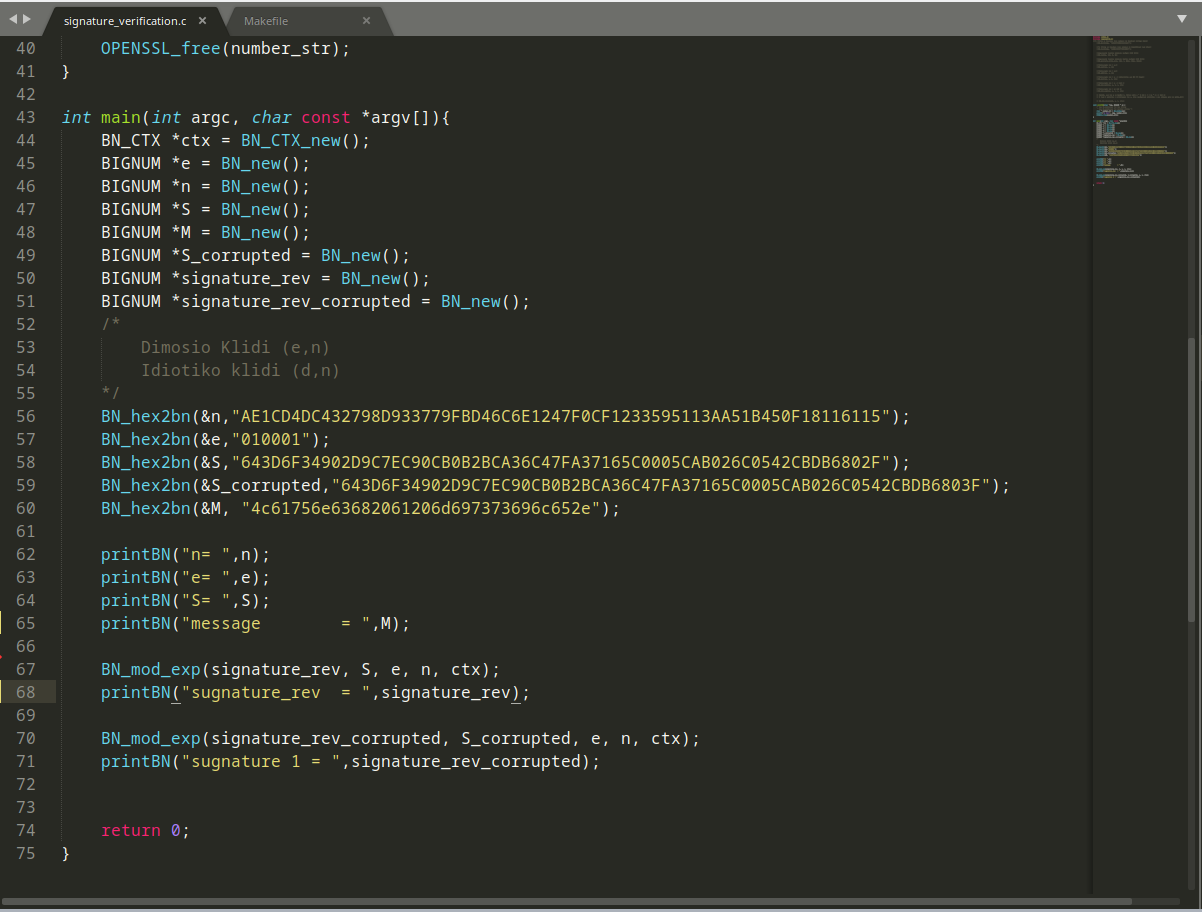
\includegraphics[width=1\textwidth]{image/image35code.PNG}		
\end{center}
\begin{center}
			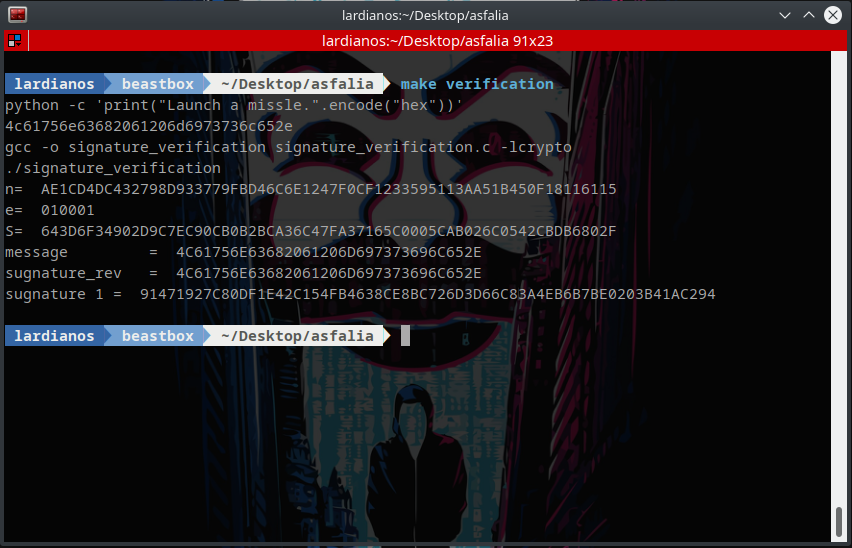
\includegraphics[width=1\textwidth]{image/image35term.PNG}		
\end{center}
\subsection{Δραστηριότητα 6: Μη αυτόµατη επαλήθευση πιστοποιητικού X.509}
\noindent

Σε αυτήν τη δραστηριότητα, θα ελέγξουµε χειροκίνητα ένα πιστοποιητικό X.509
χρησιµοποιώντας το πρόγραµµά µας. Ένα X.509 περιέχει δεδοµένα σχετικά µε ένα δηµόσιο
κλειδί και την υπογραφή του εκδότη στα δεδοµένα. Θα λάβουµε ένα πραγµατικό πιστοποιητικό
X.509 από έναν διακοµιστή ιστού, θα πάρουµε το δηµόσιο κλειδί του εκδότη του και στη
συνέχεια θα χρησιµοποιήσουµε αυτό το δηµόσιο κλειδί για να επαληθεύσουµε την υπογραφή
στο πιστοποιητικό.

\noindent
\textbf{Βήµα 1: Κατεβάστε ένα πιστοποιητικό από έναν πραγµατικό server}. Χρησιµοποιούµε τον
διακοµιστή \url{www.example.org}. Οι φοιτητές θα πρέπει να επιλέξουν διαφορετικό server που
έχει διαφορετικό πιστοποιητικό από αυτό που χρησιµοποιείται σε αυτό το έγγραφο (θα πρέπει
να σηµειωθεί ότι το \url{www.example.com} µοιράζεται το ίδιο πιστοποιητικό µε το
\url{www.example.org}). Μπορούµε να κατεβάσουµε πιστοποιητικά χρησιµοποιώντας
προγράµµατα περιήγησης ή να χρησιµοποιήσουµε την παρακάτω εντολή:

\begin{lstlisting}
$ openssl s_client -connect www.example.org:443 -showcerts
Certificate chain
0 s:/C=US/ST=California/L=Los Angeles/O=Internet Corporation for
Assigned
Names and Numbers/OU=Technology/CN=www.example.org
i:/C=US/O=DigiCert Inc/OU=www.digicert.com/CN=DigiCert SHA2 High
Assurance
Server CA
-----BEGIN CERTIFICATE-----
MIIF8jCCBNqgAwIBAgIQDmTF+8I2reFLFyrrQceMsDANBgkqhkiG9w0BAQsFADBw
MQswCQYDVQQGEwJVUzEVMBMGA1UEChMMRGlnaUNlcnQgSW5jMRkwFwYDVQQLExB3
......
wDSiIIWIWJiJGbEeIO0TIFwEVWTOnbNl/faPXpk5IRXicapqiII=
-----END CERTIFICATE-----
\end{lstlisting}
\pagebreak
\begin{lstlisting}
1 s:/C=US/O=DigiCert Inc/OU=www.digicert.com/CN=DigiCert SHA2 High
Assurance Server CA
i:/C=US/O=DigiCert Inc/OU=www.digicert.com/CN=DigiCert High
Assurance
EV Root CA
-----BEGIN CERTIFICATE-----
MIIEsTCCA5mgAwIBAgIQBOHnpNxc8vNtwCtCuF0VnzANBgkqhkiG9w0BAQsFADBs
MQswCQYDVQQGEwJVUzEVMBMGA1UEChMMRGlnaUNlcnQgSW5jMRkwFwYDVQQLExB3
......
cPUeybQ=
-----END CERTIFICATE-----
\end{lstlisting}

\noindent
Το αποτέλεσµα της εντολής περιέχει δύο πιστοποιητικά. Το πεδίο του θέµατος (η καταχώριση
που αρχίζει µε s:) του πιστοποιητικού είναι www.example.org, δηλ. αυτό είναι πιστοποιητικό
του www.example.org. Το πεδίο του εκδότη (η καταχώριση που αρχίζει µε i:) παρέχει τις
πληροφορίες του εκδότη. Το πεδίο του θέµατος του δεύτερου πιστοποιητικού είναι το ίδιο µε το
πεδίο του εκδότη του πρώτου πιστοποιητικού. Βασικά, το δεύτερο πιστοποιητικό ανήκει σε µια
ενδιάµεση CA (Certification Authority - Αρχή Πιστοποιήσεων). Σε αυτή τη δραστηριότητα, θα
χρησιµοποιήσουµε το πιστοποιητικό της CA για να επαληθεύσουµε ένα πιστοποιητικό
διακοµιστή.

\noindent
Εάν λάβετε µόνο ένα πιστοποιητικό πίσω χρησιµοποιώντας την παραπάνω εντολή, αυτό
σηµαίνει ότι το πιστοποιητικό που λάβατε υπογράφεται από µια root CA. Πιστοποιητικά από
root CA µπορούν να ληφθούν από το πρόγραµµα περιήγησης Firefox που είναι εγκατεστηµένο
στο προκατασκευασµένο VM. Επιλέξτε Edit —> Preferences —> Privacy —> και μετά
Security —> View Certificates. Αναζητήστε το όνοµα του εκδότη και κατεβάστε το
πιστοποιητικό του.


\noindent
Αντιγράψτε και επικολλήστε σε ένα αρχείο καθένα από τα πιστοποιητικά (το κείµενο µεταξύ
της γραµµής που περιέχει το “Begin CERTIFICATE" και της γραµµής που περιέχει “End
CERTIFICATE", συµπεριλαµβανοµένων των δύο αυτών γραµµών). Ονοµάστε το ένα αρχείο
c0.pem και το άλλο c1.pem.

\noindent
\textbf{Βήµα 2: Εξαγάγετε το δηµόσιο κλειδί (e, n) από το πιστοποιητικό του εκδότη}. Το Openssl
παρέχει εντολές για την εξαγωγή ορισµένων χαρακτηριστικών από τα πιστοποιητικά x509.
Μπορούµε να εξαγάγουµε την τιµή του n χρησιµοποιώντας -modulus. Δεν υπάρχει ειδική
εντολή για την εξαγωγή του e, αλλά µπορούµε να εκτυπώσουµε όλα τα πεδία και εύκολα να
βρούµε την αξία του e.

\begin{lstlisting}
For modulus (n):
$ openssl x509 -in c1.pem -noout -modulus
Print out all the fields, find the exponent (e):
$ openssl x509 -in c1.pem -text -noout
\end{lstlisting}

\noindent
\textbf{Βήµα 3: Εξαγάγετε την υπογραφή από το πιστοποιητικό του διακοµιστή}. Δεν υπάρχει
συγκεκριµένη εντολή openssl για την εξαγωγή του πεδίου υπογραφής. Ωστόσο, µπορούµε να
εκτυπώσουµε όλα τα πεδία και στη συνέχεια να αντιγράψουµε και να επικολλήσουµε το µπλοκ
υπογραφής σε ένα αρχείο (σηµείωση: αν ο αλγόριθµος υπογραφής που χρησιµοποιείται στο
πιστοποιητικό δεν βασίζεται στον RSA, µπορείτε να βρείτε ένα άλλο πιστοποιητικό).

\begin{lstlisting}
$ openssl x509 -in c0.pem -text -noout
...
Signature Algorithm: sha256WithRSAEncryption
84:a8:9a:11:a7:d8:bd:0b:26:7e:52:24:7b:b2:55:9d:ea:30:
89:51:08:87:6f:a9:ed:10:ea:5b:3e:0b:c7:2d:47:04:4e:dd:
......
5c:04:55:64:ce:9d:b3:65:fd:f6:8f:5e:99:39:21:15:e2:71:
aa:6a:88:82
\end{lstlisting}

\noindent
Πρέπει να αφαιρέσουµε τα διαστήµατα και τις άνω κάτω τελείες από τα δεδοµένα, έτσι ώστε να
έχουµε µια δεκαεξαδική συµβολοσειρά µε την οποία µπορούµε να τροφοδοτήσουµε το
πρόγραµµά µας. Οι παρακάτω εντολές µπορούν να επιτύχουν αυτόν τον στόχο. Η εντολή tr
είναι ένα βοηθητικό εργαλείο Linux για τις λειτουργίες string. Σε αυτή την περίπτωση, η
επιλογή -d χρησιµοποιείται για τη διαγραφή των ":" και "κενών" από τα δεδοµένα.

\begin{lstlisting}
$ cat signature | tr -d '[:space:]:'
84a89a11a7d8bd0b267e52247bb2559dea30895108876fa9ed10ea5b3e0bc7
......
5c045564ce9db365fdf68f5e99392115e271aa6a8882
\end{lstlisting}

\noindent
\textbf{Βήµα 4: Εξαγάγετε το σώµα του πιστοποιητικού του διακοµιστή}. Μια Αρχή Πιστοποίησης
(CA) δηµιουργεί την υπογραφή για ένα πιστοποιητικό διακοµιστή, αρχικά υπολογίζοντας το
hash του πιστοποιητικού και στη συνέχεια υπογράφει το hash. Για να επαληθεύσουµε την
υπογραφή, πρέπει επίσης να δηµιουργήσουµε το hash από ένα πιστοποιητικό. Δεδοµένου ότι ο
κατακερµατισµός δηµιουργείται πριν από τον υπολογισµό της υπογραφής, πρέπει να
αποκλείσουµε το µπλοκ υπογραφής ενός πιστοποιητικού κατά τον υπολογισµό του hash. Η
εύρεση του τµήµατος του πιστοποιητικού που χρησιµοποιείται για τη δηµιουργία του hash
είναι αρκετά δύσκολη χωρίς την καλή κατανόηση της µορφής του πιστοποιητικού.

\noindent
Τα πιστοποιητικά X.509 κωδικοποιούνται χρησιµοποιώντας το πρότυπο ASN.1 (Abstract Syntax
Notation.One), οπότε αν µπορέσουµε να αναλύσουµε τη δοµή ASN.1, µπορούµε εύκολα να
εξαγάγουµε οποιοδήποτε πεδίο από ένα πιστοποιητικό. Το Openssl έχει µια εντολή που
ονοµάζεται asn1parse, η οποία µπορεί να χρησιµοποιηθεί για την ανάλυση ενός
πιστοποιητικού X.509

\noindent
\begin{lstlisting}
$ openssl asn1parse -i -in c0.pem
0:d=0 hl=4 l=1522 cons: SEQUENCE
4:d=1 hl=4 l=1242 cons: SEQUENCE	(1)
8:d=2 hl=2 l= 3 cons: cont [ 0 ]
10:d=3 hl=2 l= 1 prim: INTEGER :02
13:d=2 hl=2 l= 16 prim: INTEGER
:0E64C5FBC236ADE14B172AEB41C78CB0
... ...
1236:d=4 hl=2 l= 12 cons: SEQUENCE
1238:d=5 hl=2 l= 3 prim: OBJECT :X509v3 Basic Constraints
1243:d=5 hl=2 l= 1 prim: BOOLEAN :255
1246:d=5 hl=2 l= 2 prim: OCTET STRING [HEX DUMP]:3000
1250:d=1 hl=2 l= 13 cons: SEQUENCE 	(2)
1252:d=2 hl=2 l= 9 prim: OBJECT :sha256WithRSAEncryption
SEED Labs – RSA Public-Key Encryption and Signature Lab 8
1263:d=2 hl=2 l= 0 prim: NULL
1265:d=1 hl=4 l= 257 prim: BIT STRING
\end{lstlisting}
\noindent
Το πεδίο που ξεκινά από το (1) είναι το σώµα του πιστοποιητικού που χρησιµοποιείται για τη
δηµιουργία του hash. Το πεδίο που ξεκινά από το (2) είναι το µπλοκ της υπογραφής. Οι
αποστάσεις τους (offsets) είναι οι αριθµοί στην αρχή των γραµµών. Στην περίπτωσή µας, το
σώµα του πιστοποιητικού είναι από το offset 4 έως το 1249, ενώ το µπλοκ υπογραφής είναι από
το 1250 έως το τέλος του αρχείου. Για τα πιστοποιητικά X.509, το offset εκκίνησης είναι πάντα το
ίδιο (δηλ. 4), αλλά το τέλος εξαρτάται από το µήκος περιεχοµένου ενός πιστοποιητικού.
Μπορούµε να χρησιµοποιήσουµε την επιλογή -strparse για να πάρουµε το πεδίο από το offset 4, 
το οποίο θα µας δώσει το σώµα του πιστοποιητικού, εξαιρουµένου του µπλοκ υπογραφής.

\begin{lstlisting}
$ openssl asn1parse -i -in c0.pem -strparse 4 -out c0_body.bin -noout
\end{lstlisting}
\noindent
Μόλις λάβουµε το σώµα του πιστοποιητικού, µπορούµε να υπολογίσουµε το hash του
χρησιµοποιώντας την ακόλουθη εντολή:

\begin{lstlisting}
$ sha256sum c0_body.bin
\end{lstlisting}
\noindent
\textbf{Βήµα 5: Επαληθεύστε την υπογραφή}. Τώρα έχουµε όλες τις πληροφορίες,
συµπεριλαµβανοµένου του δηµόσιου κλειδιού της ΑΠ, της υπογραφής της ΑΠ και του σώµατος
του πιστοποιητικού του διακοµιστή. Μπορούµε να εκτελέσουµε το δικό µας πρόγραµµα για να
ελέγξουµε αν η υπογραφή είναι έγκυρη ή όχι. Το Openssl παρέχει µια εντολή για την
επαλήθευση του πιστοποιητικού για εµάς, αλλά οι φοιτητές καλούνται να χρησιµοποιήσουν και
τα δικά τους προγράµµατα για να το κάνουν.

\subsection*{Απάντηση:}

\noindent
Ως πηγή για τα certificates θα χρησιμοποιήσουμε το www.google.com επομένως
εκτελούμε την εντολή και μας παρουσιάζονται τα πιστοποιητικά του google.
\begin{center}
			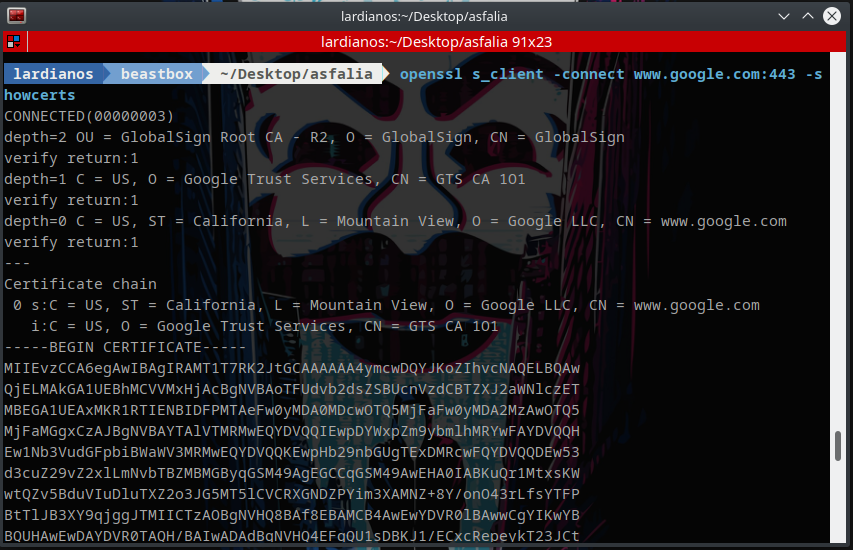
\includegraphics[width=1\textwidth]{image/image36term1.PNG}		
\end{center}
\noindent
Επιλέγουμε από το BEGIN εως το END και τα αποθηκεύουμε σε δυο αρχεία c0.pem και c1.pem
\begin{center}
			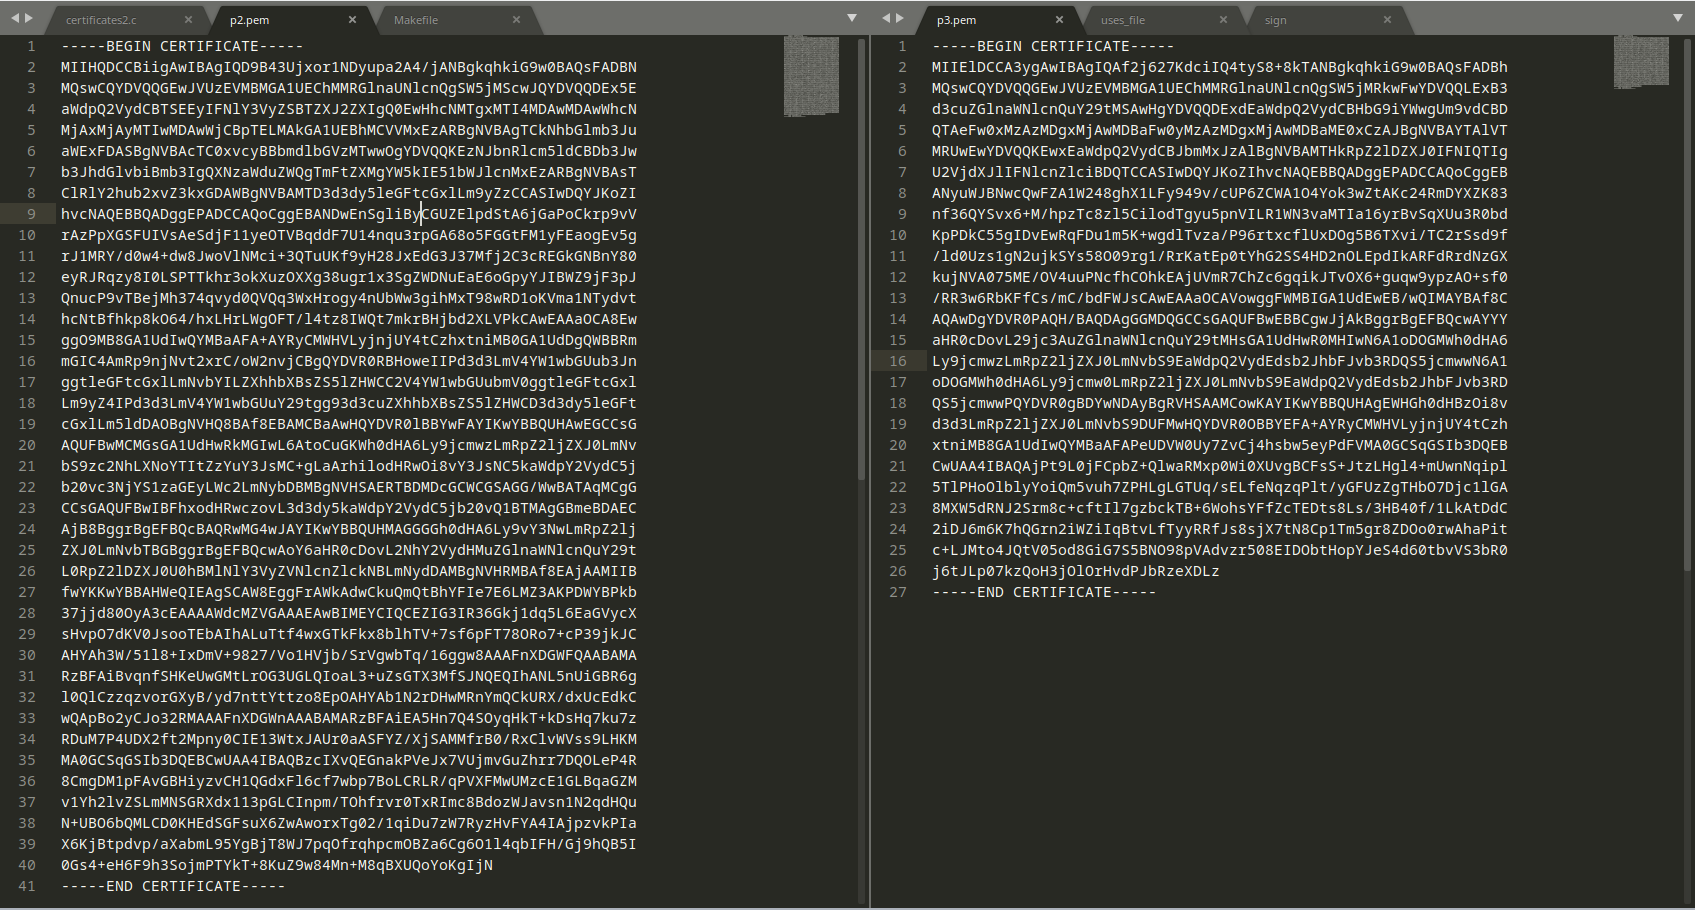
\includegraphics[width=1\textwidth]{image/image36cert.PNG}		
\end{center}
\noindent
Εκτελούμε την παρακάτω εντολή και περνούμε το ένα μέρος του δημοσίου κλειδιού (n)
\begin{center}
			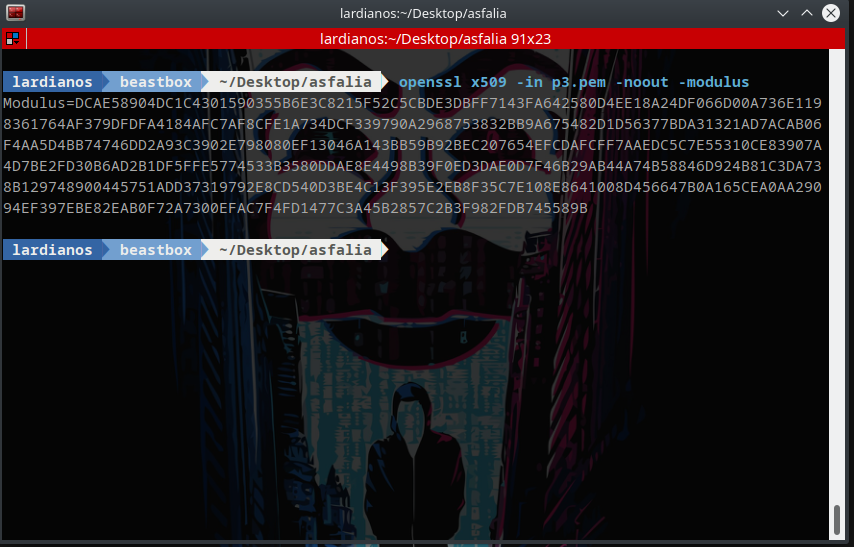
\includegraphics[width=1\textwidth]{image/image36term2.PNG}		
\end{center}
\noindent
Για το άλλο μέρος του κλειδιού (e) εκτελούμε τη παρακάτω εντολή και βρίσκουμε 
το σημείο που γραφή Exponent και το κρατάμε κάπου και αυτό.
\begin{center}
			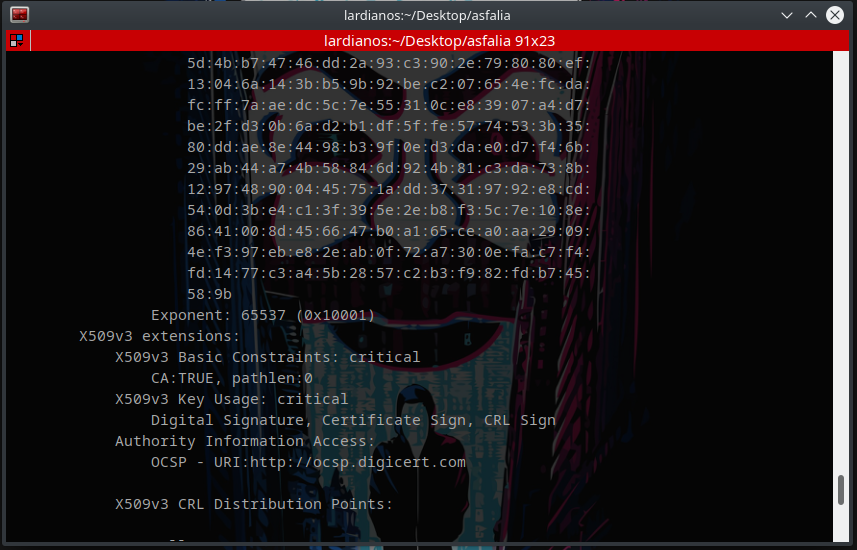
\includegraphics[width=1\textwidth]{image/image36term3.PNG}		
\end{center}
\noindent
Εκτελούμε την παρακάτω εντολή αυτήν την φορά για το αρχείο c0.pem
και βρίσκουμε το σημείο που γραφή Signature Algorithm και το αντιγράφουμε και αυτό σε ένα αρχείο
\begin{center}
			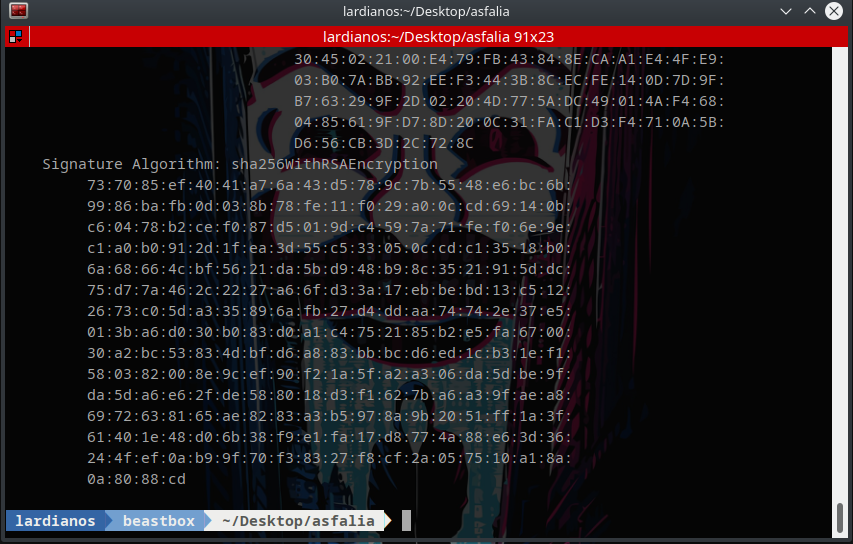
\includegraphics[width=1\textwidth]{image/image36term4.PNG}		
\end{center}
\noindent
Με την παρακάτω εντολή αναφέρουμε όλα τα κενά και της : που υπάρχουν 
\begin{center}
			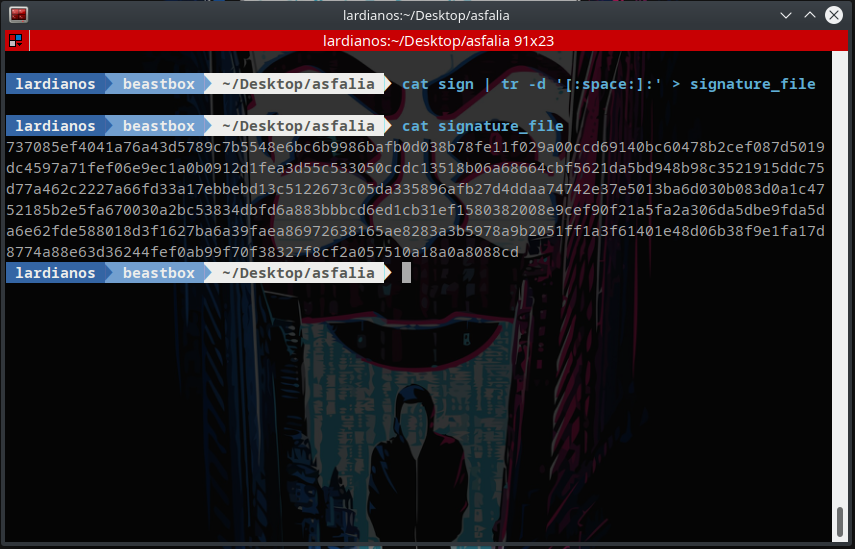
\includegraphics[width=1\textwidth]{image/image36term5.PNG}		
\end{center}
\noindent
με της παρακάτω εντολές διαχωρίζουμε το σόμα του πιστοποιητικού χωρίς την υπογραφή.
\begin{center}
			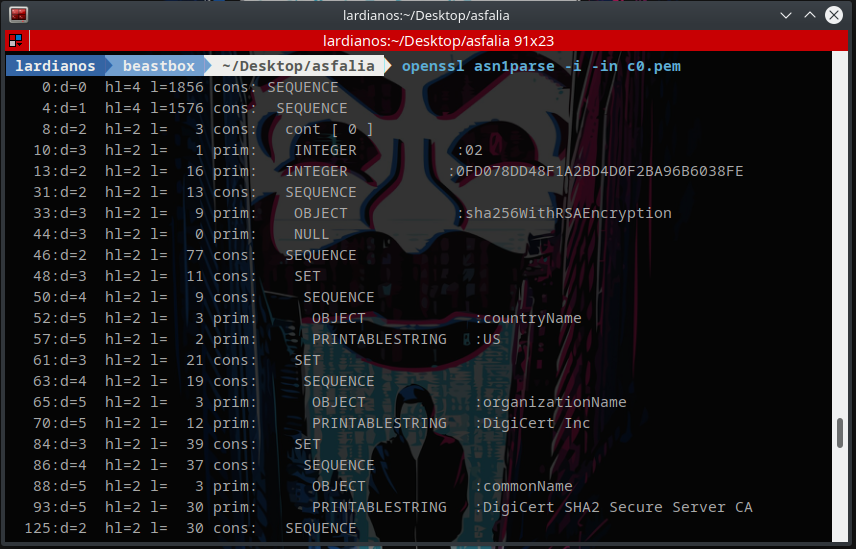
\includegraphics[width=1\textwidth]{image/image36term6.PNG}		
\end{center}
\begin{center}
			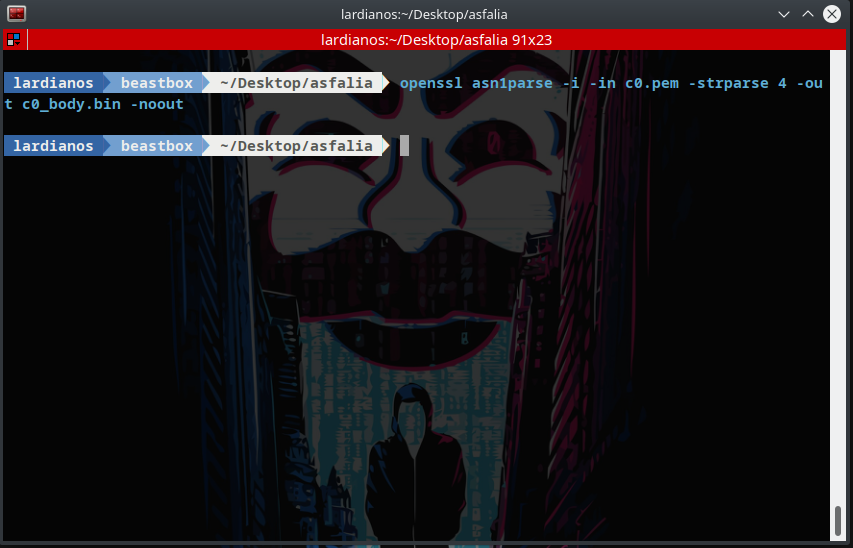
\includegraphics[width=1\textwidth]{image/image36term7.PNG}		
\end{center}
\noindent
Από το σόμα του πιστοποιητικού υπολογίζουμε το hash.
\begin{center}
			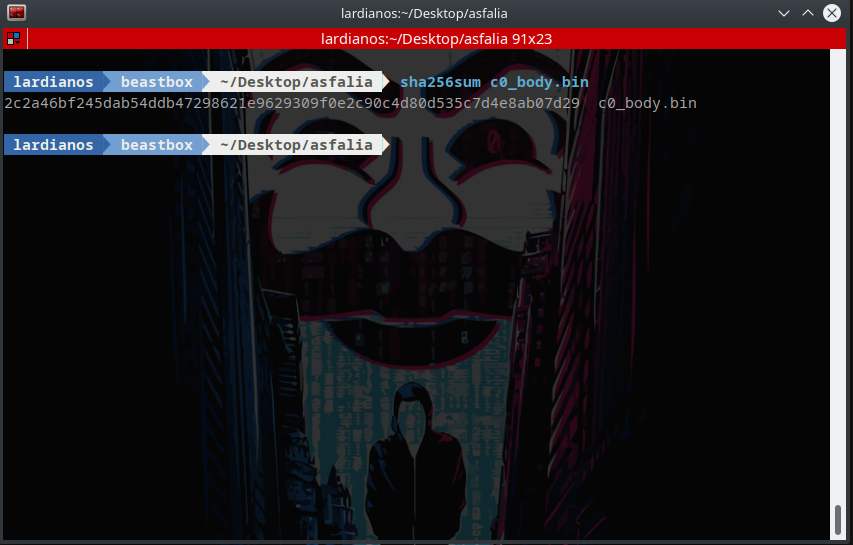
\includegraphics[width=1\textwidth]{image/image36term8.PNG}		
\end{center}
\noindent
και πλέων έχουμε όλες της πληροφορίες που χρειαζόμαστε για να κάνουμε την επαλήθευση.
\begin{center}
			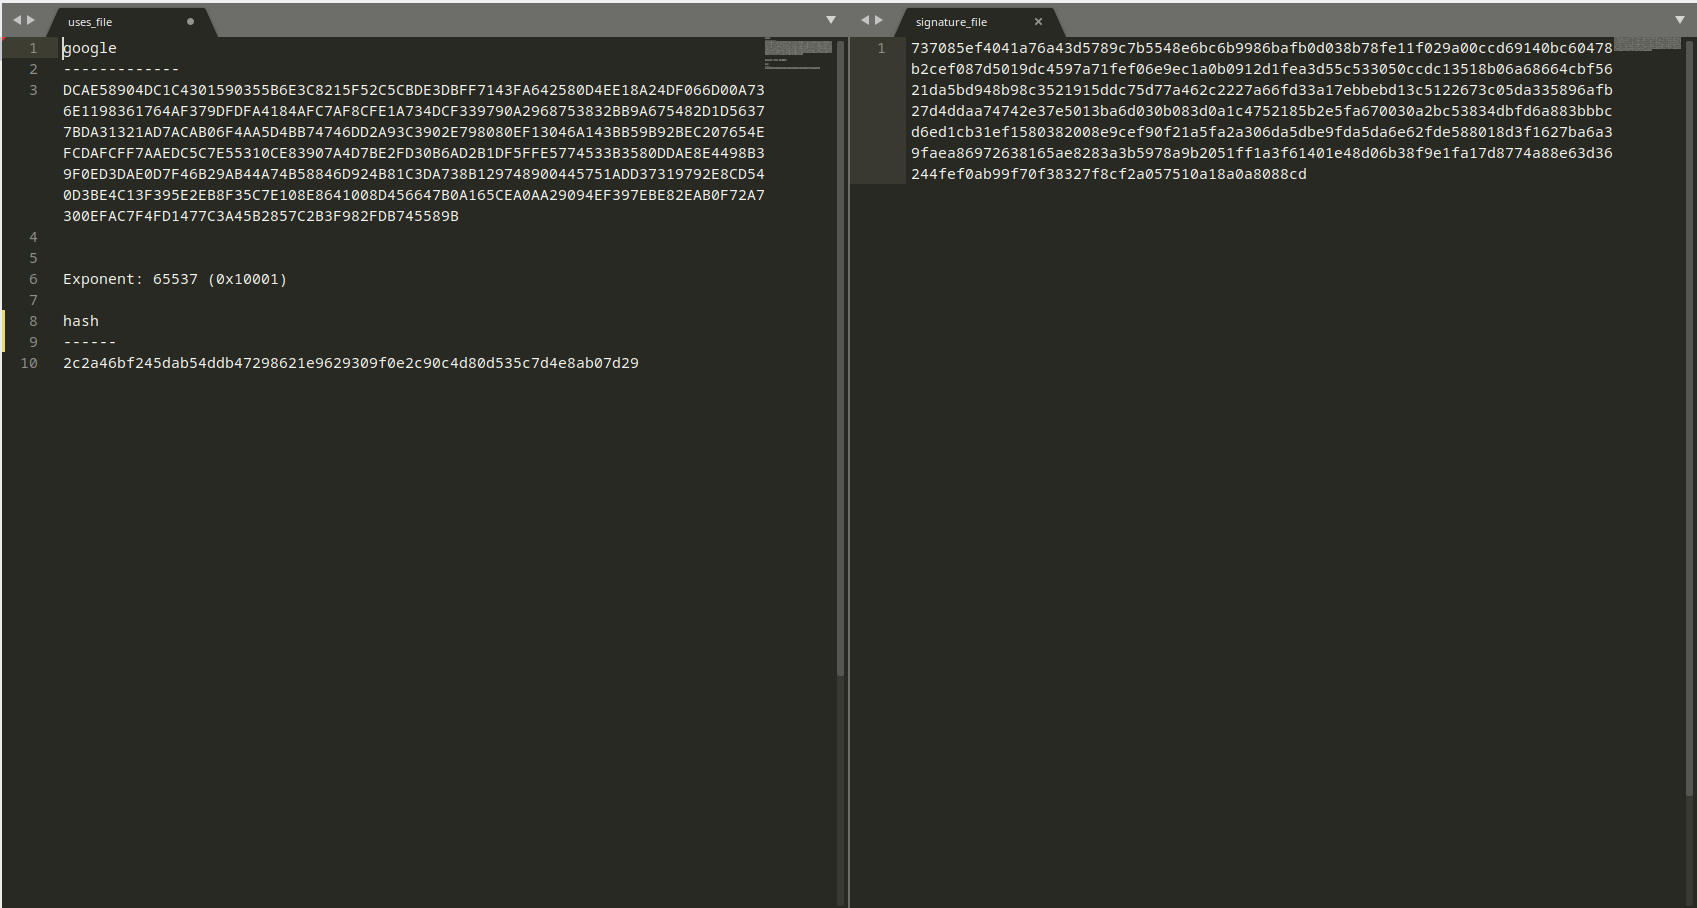
\includegraphics[width=0.9\textwidth]{image/image36term9.PNG}		
\end{center}
\noindent
Της περνάμε στο πρόγραμμα μας 
\begin{center}
			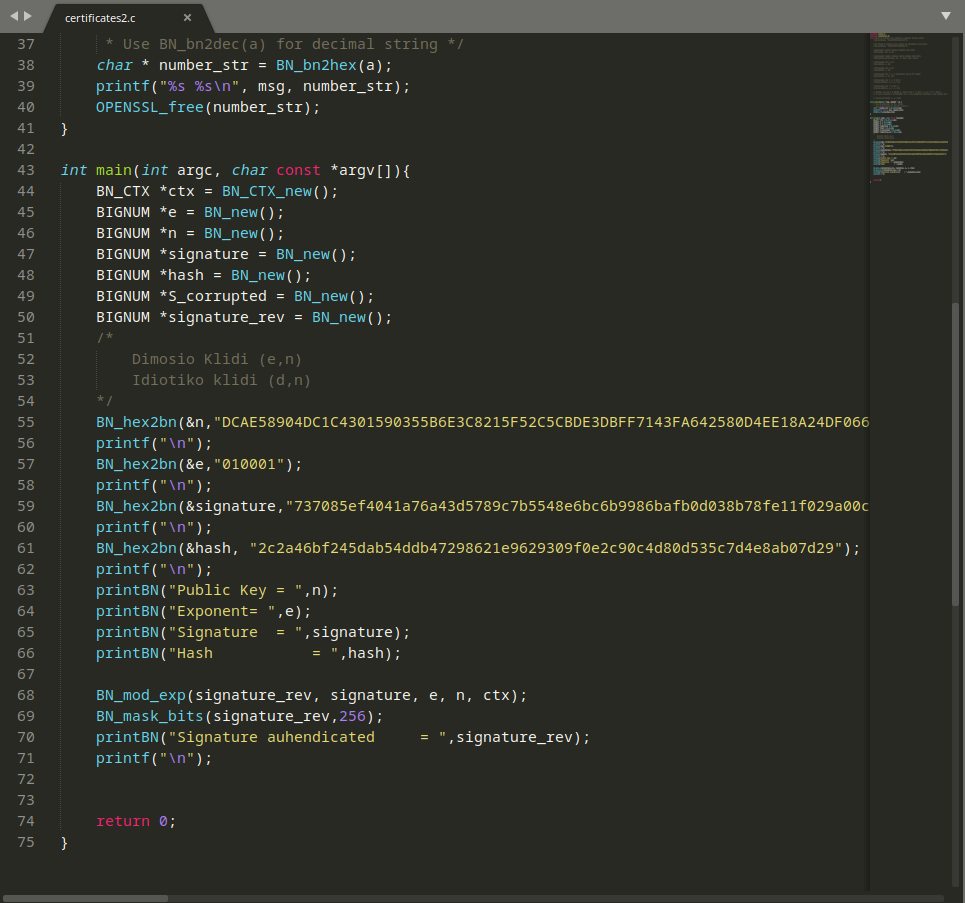
\includegraphics[width=0.9\textwidth]{image/image36code.PNG}		
\end{center}
\pagebreak
\noindent
Το εκτελούμε και παρατηρούμε ότι το hash που υπολογίσαμε είναι ίδιο με αυτό 
που προέκυψε από την αποκρυπτογράφηση επομένως η επαλήθευση ήταν επιτυχής!
\begin{center}
			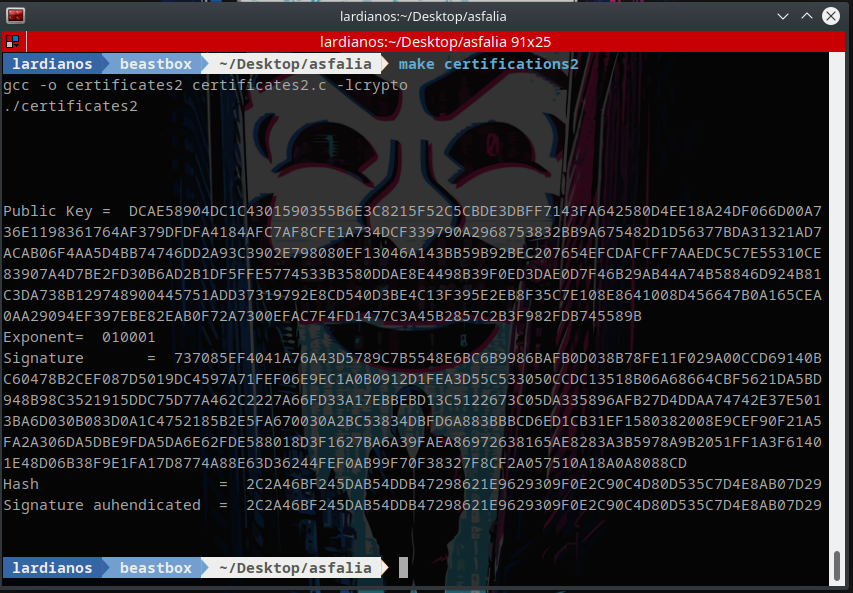
\includegraphics[width=1\textwidth]{image/image36term10.PNG}		
\end{center}
\pagebreak
\noindent
Τέλος για την ευκολία μας μπορούμε να δημιουργήσουμε ένα Makefile σαν το παρακάτω που μας γλιτώνει χρόνο
στα compile και execute τον προγραμμάτων μας για της δόκιμες που κάναμε.
\begin{center}
			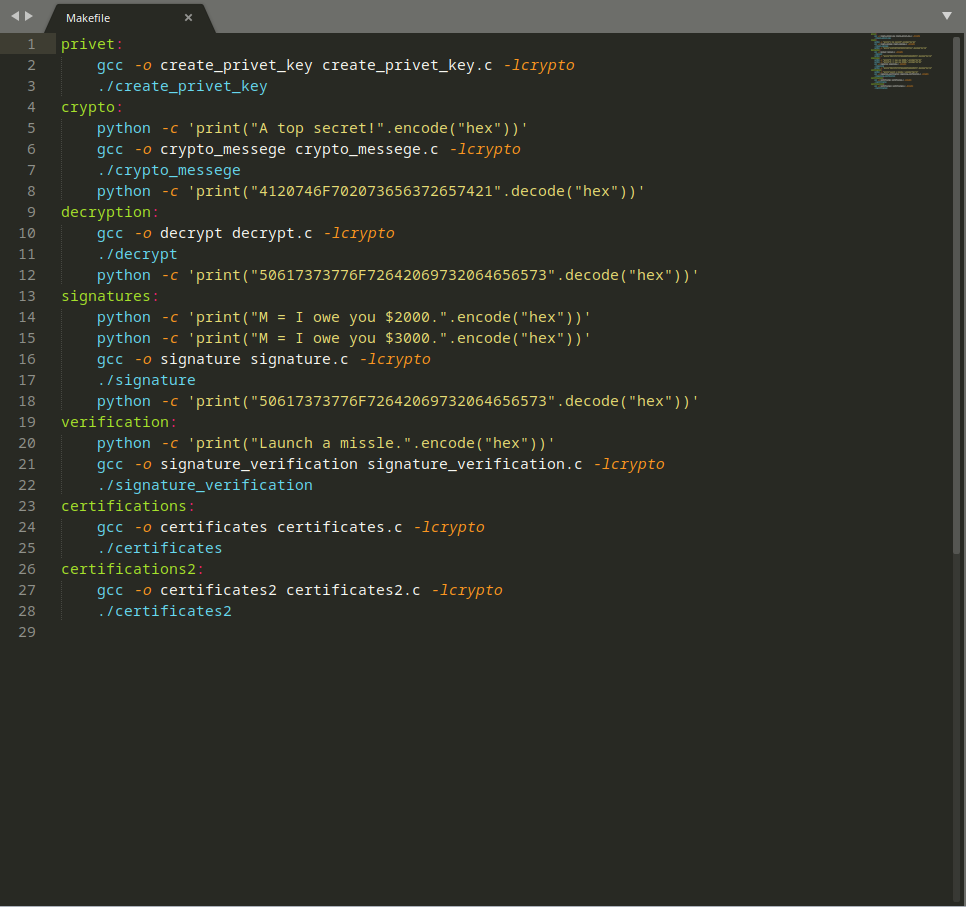
\includegraphics[width=1\textwidth]{image/makefile.PNG}		
\end{center}